\documentclass{article}
\usepackage[background]{genesys}
\title{Vitia 2.0}
\author{Kaleb Poole}
\date{July 2019}
\graphicspath{{./img/}}
\setlength{\parindent}{0cm}
\newenvironment{SpellTable}[0]{%
    \begin{GenesysTable}{|X[l]|X[4l]|X[l]|}
    \hline Effect Name & Effect & Difficulty Increase \\ \hline
  }
{\end{GenesysTable}}
\newenvironment{WeaponTable}[0]{%
    \begin{GenesysTable}{|X[l3]|X[l]|X[l]|X[l]|X[l1.5]|X[l]|X[l6]|}
    \hline Weapon Name & Type & Damage & Critical & Range & Price & Modifiers \\ 
    \hline
  }
{\end{GenesysTable}}
\newenvironment{Figure}
  {\par\medskip\noindent\minipage{\linewidth}}
  {\endminipage\par\medskip}
\newcommand{\WeaverPrereq}{\textit{This talent requires your character to be able to cast spells with Weaving to benefit from it.}\\}
\newcommand{\NaturalPrereq}{\textit{This talent requires your character to be able to cast spells with Manaflow to benefit from it.}\\}
\newcommand\CasterPrereq{\textit{This talent requires your character to be able to cast spells to benefit from it.}\\}
\newcommand\Simple{Simple [-]}
\newcommand\Easy{Easy [\Purple[1]]}
\newcommand\Average{Average [\Purple[2]]}
\newcommand\Hard{Hard [\Purple[3]]}
\newcommand\Daunting{Daunting [\Purple[4]]}
\newcommand\Formidable{Formidable [\Purple[5]]}
\newcommand\Impossible{Impossible [\Purple[5]]}
\newcommand\Nocast[1]{Natural casters who use #1 magic cannot cast these spells.}
\setcounter{tocdepth}{2} 
\begin{document}
\begin{multicols}{2}
\tableofcontents
\end{multicols}
\newpage
\section{Introduction}
\section{Crime and Punishment}
\begin{multicols}{2}
\subsection{Going to Jail}
Crimes in Vitia are often left unpunished, that being said there is a trick to getting away with murder. All you have to do is realise that most of the police officers work for a syndicate, usually the one that controls the area you've been arrested in. If you work for that syndicate too, they probably won't arrest you, or they'll let you off. If you don't however, either they want to random you back to your boss, In which case your in for a bad time, or they don't, in which case a small bribe will probably solve your problem unless you've pissed them off. If they do chose to detain you, you're probably going to end up in a rug floating down the river, or working manual labour at gunpoint, whichever is better for the syndicate.\par
\columnbreak
\subsection{Bounties}
It is worth noting there are worse punishments than being arrested. Notably people like to put bounties out when they want someone punished. Bounties aren't just dead or alive, often you find bounties to break people's legs, or to kidnap and torture a target. Bounties are functionally just a public job posting. They're a good way for new groups to make a name for themselves and get the opportunity to be invited on jobs that require more discretion, and higher pay.
\end{multicols}
\section{The Factions}
\begin{multicols}{2}
\subsection{The Syndicates}
There are 8 large syndicates that operate within Vitia, each of which are known by an associated colour that matches the crown their leaders, dubbed 'Kings', bear.

\begin{Figure}
\centering
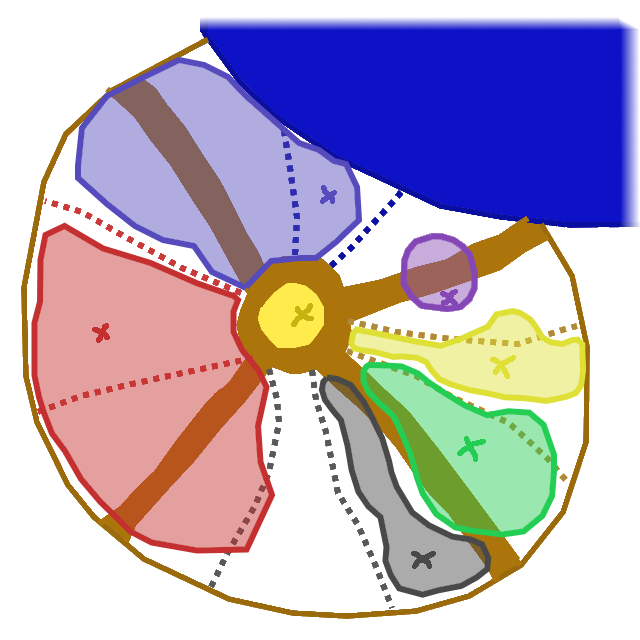
\includegraphics[width=\linewidth]{Gangs.png}
A map of the Syndicate's territories within Vitia
\end{Figure}
\vbox{
\subsubsection{The Kings and Their Crowns}
Each of the eight syndicates has a king, who bears a crown. These crowns look like simple three pointed crowns tattooed onto the kings left forearm (or elsewhere, if there is no such arm). However they are much more than a tattoo. The exact nature of the crowns is unknown but they allow a king to give power to their underlings, in the form of increasingly large and ornate bands of colour around a persons left wrist.\par
When a King is slain, the Crown is \textit{supposed} to be inherited by whoever killed the king that bore it, however in certain cases this does not occur, in which case the crown goes to someone within the city that shares the king's mentality at death.\par
Because the crowns allow the kings to give their people power, whenever a crown goes missing, which isn't all that often, the syndicate is weakened and often actively looking for whoever has the crown, so that they can regain the power they lost when the last king died.\par
There is an urban legend that if anyone ever manages to possess all eight crowns then they can become a literal god. Because of this, and the fact that they're direct business competitors, the kings do not trust each other, and actively conceal their identities.
}\vbox{
\subsubsection{The Red Syndicate}
The Red Syndicate, based in Vitia's western industrial district they control the largest portion of the city, both in terms of area and population. They primarily make money by manufacturing and selling weapons, magical and mundane, across the world. Under the table contracts with governments, shady trades with pirates in the south china sea, morally grey deals with rebels and freedom fighters. If you want weapons, and you've got money, the Red Syndicate will provide.\par
The Red King, however, was recently killed by \textit{The King Slayer} which subsequently leaves the syndicate looking for whoever inherited the crown.
}\vbox{
\subsubsection{The Blue Syndicate}
The Blue Syndicate is based in Vitia's northern docks and directly contest The Red Syndicate for territory and the claim of being the largest syndicate. They smuggle drugs and other black market goods into the rest of the world, if you want to move a ship in Vitia you'd better know someone in the blues, or be really quiet about it.\par
The Blue King claims to be clairvoyant, and is allegedly able to see into the future, although he vehemently denies any such claims. He is a business man first, and a King second, he will often sell his own people to their enemies if he thinks it's a better decision than protecting them.
}\vbox{
\subsubsection{The Green Syndicate}
The Green Syndicate is based in Vitia's richer eastern residential district and is in direct conflict with the Yellow and Black syndicates for territory. The services they provide are very broad, often described more like private military contractors than a crime syndicate. The greens offer several services to people in the city, and the wider world. Including arbitrating wireless kill switches, assassinations and espionage, ransoms, money laundering, and many more sketchy business ventures.\par
The Green King is surprisingly young given his occupation, the exact nature of his magic isn't totally known, but he's been observed to walk through walls, teleport himself and others, and alter the properties of things around him. He's ambitious and greedy, claiming to have already killed The Silver King, with the crown to prove it, although he refuses to give a silver mark to anyone in his employ.  
}\vbox{
\subsubsection{The Yellow Syndicate}
The Yellow Syndicate is based in Vitia's richer eastern residential district and as such is in conflict with the Green Syndicate for territory. They provide Vitia's 1\% with recreational services, access to designer drugs (often purchased from the Blue Syndicate), high end whores, and debased sex clubs all fall under their umbrella as well as several more things. When it comes to pleasure the Yellow Syndicate have things sorted.\par
The Yellow King is an aloof woman. She's known for flights of fancy and generally being a nightmare to predict and work with. She's quite open about her ability to manipulate minds in the form of illusions. She claims that all she wants is for everyone to get along, although that doesn't stop her from skinning people who cross her.
}\vbox{
\subsubsection{The Black Syndicate}
The Black Syndicate are a weird bunch, they're based in the cities southern residential district, which houses the more middle class folk who can afford not to squat; They contest the Green Syndicate for territory in the eastern district. Calling the Black Syndicate a syndicate is generous, they share more features with a cult than an organised crime ring. Most of their income comes from protection rackets and 'generous donations'.\par
The Black King is a force to be reckoned with well known for making her enemies disappear never to be seen again, the only people who have survived such a 'black bagging' claim to have walked through a door only to find themselves in a poorly lit black room with a single heavy metal door. The Black King herself is manipulative, she made excellent use of religious rhetoric to build up her cult and continues to use it to this day. She claims to be an agent of 'The Watcher' whatever the hell that is.
}
\begin{Figure}
\centering

\includegraphics[width=0.5\linewidth]{Watcher.png}
\\The Watcher's Symbol. Often seen inside the Black Syndicate's territories
\end{Figure}
\vbox{
\subsubsection{The Purple Syndicate}
The Purple Syndicate is the smallest operational syndicate, they lay claim to a small part of the docks and eastern residential districts. The Purple Syndicate suffered a brutal defeat at the hands of the late Red King and ended up unable to maintain control of their territory, they fell from being the most affluent and powerful of the syndicates to the least in a few short months. When \textit{The King Slayer} killed the Purple King, it was salt in the wound. The few remaining members of the syndicate can only hope that the new king, wherever they are, will make things better. 
}\vbox{
\subsubsection{The Gold Syndicate}
The Gold Syndicate is hardly a syndicate, they control a single building in the city centre, a theatre, and have only a few dozen people in their roster. The Gold King's seat is used to host semi-regular meetings between the Syndicates, in the form of a masquerade ball.\par
The Gold King himself is a very powerful mage, although wholly unmotivated to use his power for nought other than making sure that there are no fights inside his theatre. The Gold King has sat on his throne for far longer than any mortal should, his records go back two centuries to Vitia's Founders. It is well known that he has ties to the Founder's Foundation, although the details of this relationship is a closely guarded secret.
}\vbox{
\subsubsection{The Silver Syndicate}
The Silver Syndicate is even less of a syndicate than the Gold Syndicate, which is to say it doesn't exist. The Silver King is missing, dead if the Green King is to be believed. This being said, behind closed doors and certainly not on record, the Gold King has said that he is certain that his old friend, the Silver King, cannot be dead.\par
The Silver King is as old as the Gold, if not slightly older. They're stood side by side, crowns visible if you squint, in the background of the photo that shows Vitia's opening ceremony just over two centuries ago.
}\vbox{
\subsection{Witches}
Witches in Vitia either operate alone, or with one of two covens. There's the \textbf{Benecci} coven and the \textbf{Malochio} coven. The Benecci are generally considered to be philanthropic, or at least not malicious. They primarily live off their own backs, growing their own food and selling recreational drugs as well as mundane healing services. The Benecci provide a great deal of support for the homeless in the industrial district that don't rely on the Red Syndicate. The Malochio on the other hand are less benign, secretive and dangerous they sell black magic to anyone with the money, acting as assassins and kidnappers, selling weapons and poisons they seek to profit off of the conflict generated by the syndicate's fighting. The Malochio are among the few groups that know how to produce void dust.
}\vbox{
\subsection{Zed's Bar}
Not really a faction, but a very important player to consider, Zed is something not quite human. He literally eats sins for power, so naturally he runs a bar that doubles as a den of debauchery. Zed's exceptionally well connected and affluent, he serves as one of the only ways to smuggle things into and out of Vitia without using the Blue Syndicate's assets.
}\vbox{
\subsection{Founder's Foundation}
The Founder's Foundation, or FF for short, are the closest thing Vitia has to a non-corrupt police department. Ran by the four eldest direct descendants of Vitia's founders, the FF seeks to ensure the gang warfare doesn't escalate too far. They use their secret police as a threat to extract 'taxes' from the city's various extra-judiciary organisations, as well as receiving actual taxes from the legal establishments inside Vitia. They are effectively Vitia's government.
}\vbox{
\subsection{The Kessler Group}
In a building where there is nothing built. in a room where there is no space, meets the group that doesn't exist.\par
The Kessler Group is more or less unknown by outsiders, they rarely communicate with each other, and meet even less frequently. The members of the Kessler Group are all scientists, of some description or another, who value knowledge above petty things like morals and money. They often fight amongst themselves to prove their worth to the group's founder. Doctor William Douglas Kessler. Doctor Kessler discovered how to perform a fully functional brain transplant before he turned 30. Since then he has lived 120 years in 8 different  bodies, the members of the Kessler Group seek his approval in exchange for the promise that they too can receive such a transplant to extend their own lives. Kessler, on the other hand, is looking for a way to achieve true immortality, to avoid the reaper's gaze.
}\vbox{
\subsection{Reapers}
Less a faction, more a force of nature, Reapers are monsters that exist solely to cut off lives that should have ended years ago. Most people will never see one, and nobody has ever seen two. They possess the rare ability to manipulate souls, or a functional equivalent, and as such when they decide you are going to die. You die.
}\vbox{
\subsection{Witch Hunters}
Best thought of as the international secret police for mages. Witch hunters were first created at some point in the 15th century by a mage who managed to splice Reaper DNA into that of a human, although he didn't know that was what he'd done. The result is humans who are extremely well tuned to combat mages. By blood a Witch Hunter can never use magic, although they are exceptionally resistant to it. As an organisation the Witch Hunters aim to prevent mages from growing too powerful for the environment they live in. Mostly they work outside of Vitia, and the few times they have intervened a king has died. Most recently, the King Slayer is an ex Witch Hunter who retired after bringing low the Purple and Red Kings.
}
\end{multicols}
\section{Inside Vitia}
\begin{multicols}{2}
\subsection{Links}
Links are how people get into and out of Vitia, they are undetectable save for when you travel through them and you relocate from Vitia, the exact location of which is unknown, to wherever the link leads. Often links are one-way and rely on certain psychological factors to function, such as not knowing your current geographical location, actively looking for Vitia, and other such things. 
There are currently three known always-active, two-way, links being from just over the northern horizon to the Bermuda triangle; 10 miles north-east to the south-china sea, and finally 30 miles south to rural England. Attempting to leave the city by travelling in a direction until something is found, either leads you in circles or through some other link.
\subsection{The Districts}
Vitia consists of five main districts, each of which serves a different roles in the city. Unfortunately Vitia exists in a state of perpetual underpopulation, partially due to rampant gang violence and partially due to the city's magical nature.
\subsubsection{The Fire District}
Located on the western side of Vitia the fire district consists largely apartment buildings, abandoned by paying citizens in favour of more desirable housing in the Stone and Wind districts, and manufacturing facilities. The apartment buildings being abandoned is not technically true, as there are a fair few squatters who are unwilling or unable to live in the other districts. The Red Syndicate calls the fire district home and makes excellent use of the factories that are not used by the Founder's Foundation and other legitimate businesses.
\subsubsection{The Water District}
The most appropriately named district, the Water District is located north of Vitia, by the coast. The water district consists largely of warehouses with a smattering of bars and clubs
\subsection{Subterranean Sewer System}
The sewers in Vitia are dangerous and labyrinthine, due to some quirk of magic they are constantly shifting and moving which makes mapping and navigating hard enough even if they weren't full of various creatures capable of wielding magic and claw equally well. Malochio witches have been known to use the city's sewers to travel around unmolested, although how they navigate the ever-changing mass of tunnels is unknown. Allegedly the tunnels contain some hidden links to various rivers across the globe, there is anecdotal evidence of links to the Ganges, the Nile, and the Amazon. 
\end{multicols}
\section{Character Creation}
\subsection{Archetypes}
\subsection{Careers}
\begin{multicols}{2}
\vbox{
\subsubsection{Paragon}
Paragons are natural leaders, they stay calm and collected in tense situations able do deescalate a conflict to stop bullets from being fired. They know the rhetoric to get what they want, and they know how to get keep their team cohesive. Whether they should be trusted is a complicated question, but it normally looks like they should.\par
A Paragon counts the following skills are career skills: \textbf{Charm, Coercion, Cool, Leadership, Negotiation, Discipline, Ranged (Light), Perception}\par
A Paragon also starts with Heavy Clothing and a Revolver, in addition to £200
}\vbox{
\subsubsection{Arcanist}
Arcanists aren't explicitly mages, however they certainly know how magic works. They know how to stop a gunshot wound from getting infected and what a mage can do to ruin your day. Arcanists are smart people who can save your life in more ways than one. Arcanists make for good artificers, if they're magically inclined.\par
An Arcanist counts the following skills as career skills: \textbf{Knowledge (Mundane), Knowledge(Mana), Cool, Discipline, Alchemy, Medicine, Streetwise, Vigilance}\par
An Arcanist starts with Heavy Clothing and £250
}\vbox{
\subsubsection{Engineer}
Engineers are drivers and mechanics. They'll rig up a car bomb, or disable security cameras. Engineers are more combat ready than Arcanists but aren't as well versed in magical knowledge. Engineers won't be able to make powerful arcane artifacts, but they can mass produce grenades in the right situations.\par
An Engineer counts the following skills as career skills: \textbf{Knowledge (Mundane),  Mechanics, Driving, Ranged (Light), Resilience, Streetwise, Computers, Perception}\par
An Engineer starts with Heavy Clothing, A Flash Grenade, and £200
}\vbox{
\subsubsection{Marksman}
Marksmen are dedicated shooters, snipers and riflemen. A Marksman can get into position and watch for the perfect opportunity to take a shot. People that have walked away from a sniper ambush will tell you that a marksman on a rooftop is one of the most terrifying things you'll ever see, or not as it stands.\par
A Marksman counts the following skills are career skills: \textbf{Streetwise, Skulduggery, Ranged (Heavy), Ranged (Light), Cool, Perception, Stealth, Discipline.}\par
A Marksman starts play with Combat Rigging, an Assault Rifle, and £50. They can trade their assault rifle and combat rigging for a Sniper Rifle instead.
}\vbox{
\subsubsection{Soldier}
Soldiers are the grit that makes Vitia work. They get stuff done with startling efficiency, barely flinching when shots are fired able to calmly assess the most important target and do what needs doing to complete their mission.\par
A Soldier counts the following skills as career skills: \textbf{Melee, Ranged (Heavy), Streetwise, Perception, Resilience, Vigilance, Driving, Athletics.}\par
A Soldier starts with Combat Armour, a Shotgun, and £50
}\vbox{
\subsubsection{Assassin}
Assassin are a mix of stealth and deadliness like no other. Assassins can sneak, climb, and talk their way into almost anywhere and once they're there they can slip a knife between someone's ribs and get out before anyone even notices. If you've earned an Assassin's ire, sleep with one eye open.\par
An Assassin counts the following skills as career skills: \textbf{Melee, Perception, Athletics, Deception, Ranged (Light), Stealth, Coordination, Streetwise.}\par
An Assassin starts with Heavy Clothing, A Military Knife, A Revolver and £150
}\vbox{
\subsubsection{Thief}
Thieves are quiet and light handed. They've got sharp eyes and a quick wit, a Thief will always be on their toes, and keep you on yours they wield a silver tongue as well as a knife or a gun.\par
A Thief counts the following skills as career skills: \textbf{Stealth, Charm, Deception, Melee, Ranged (Light), Streetwise, Skulduggery, Perception.}\par
A Thief starts with Heavy Clothing, A Commercial Knife, A Revolver, and £200
}\vbox{
\subsubsection{Artificer}
Artificers are more magically inclined even than Arcanists, they understand both how magic and mechanics works. Able to make intricate arcane devices as well as mechanical tools. An artificer is always a useful addition for their unique understanding.\par
An Artificer counts the following skills as career skills: \textbf{Mechanics, Knowledge (Mana), Ranged (Light), Perception, Driving, Operating, Perception, Vigilance.}\par
An Artificer starts with a Heavy Coat, a Revolver, and £200 
}
\end{multicols}
\subsection{Talents}
\begin{multicols}{2}
A note, many talents allow you to reduce the difficulty of Weaving and Manaflow checks, these effects remove \Purple[1] and do not downgrade the difficulty. Apply them before any difficulty upgrades, additionally these effects cannot reduce the difficulty of a check by more than half its initial difficulty

\Talent
{Careful Aim}
{1}
{Passive}
{Yes}
{You can aim one additional time per rank in Careful Aim (3 -> 4 -> 5)}

\Talent
{Arcane Study}
{1}
{Passive}
{Yes}
{\WeaverPrereq Select two additional effects. You can add them to spells}

\Talent
{Focused Aim}
{2}
{Passive}
{Yes}
{For each rank you have in Dead Eye, your first aim action counts as two aim actions (so your first 1 action, 2 actions etc.)}

\Talent
{Focused Aim}
{2}
{Active (Manoeuvre)}
{Yes}
{Once per encounter, you may use this manoeuvre to immediately take a number of aim manoeuvres equal to your ranks in Dead Eye (ignoring the normal limit on manoeuvres)}

\Talent
{Gather Mana}
{2}
{Active (Manoeuvre)}
{Yes}
{\CasterPrereq
Activate this talent to gain \Blue[1] on your next Manaflow or Weaving check, stacks up to twice your ranks in Gather Mana, if you take an action to do anything other than cast a spell, lose this bonus.}

\Talent
{Preferred Spell}
{2}
{Passive}
{No}
{\WeaverPrereq
Select a spell (A specific combination of additional effects). When you cast this spell, reduce the difficulty by \DifficultyDie}

\Talent
{Empowered Transformation}
{3}
{Passive}
{Levelled}
{\textit{Your character must have purchased Transformation from Terrinoth to benefit from this talent.}
Pick one of the pieces of equipment or abilities listed below. Whilst transformed your character has that equipment or ability. When you take multiple levels of this talent, pick another. These effects are biological and can't be given away.
}
\end{multicols}

\begin{GenesysTable}{|X[l3]|X[l]|X[l]|X[l]|X[l1.5]|X[l6]|}
Weapon Name & Skill & Damage & Critical & Range & Qualities\\ 
\hline
Venomous Fangs & Brawl & +1 & 3 & Engaged & Burn 2, Pierce 3\\ 
\hline
Crushing Limbs & Brawl & +3 & 4 & Engaged & Concussive 1, Inaccurate 2 \\ 
\hline
Scything Claws & Melee & +2 & 2 & Engaged & Blast 3, Vicious 2 \\ 
\hline
Bone Spines & Ranged (Light) & 5 & 2 & Short & Pierce 1, Vicious 3 \\ 
\hline
Acid Cannon & Ranged (Heavy) & 12 & 4 & Medium & Burn 6, Prepare 5, Inaccurate 3 \\ 
\hline
\end{GenesysTable}
\begin{multicols}{2}
\Talent
{Advanced Preferred Spell}
{4}
{Passive}
{No}
{\textit{Your character must have purchased Preferred Spell to benefit from this talent.} 
Reduce the difficulty of casting your preferred spell by up to \Purple[2], this effect replaces Preferred Spell}

\Talent
{Second Nature}
{5}
{Active (incidental)}
{No}
{\NaturalPrereq
When you get this talent, pick a spell. If you would ever cast this spell for a difficulty of \Purple[1] or less you may instead use this talent to act as if you had rolled a number of \Success and \Advantage equal to your ranks in Manaflow. You still have to spend 2 strain}

\Talent
{Versatile Targeting}
{1}
{Passive}
{No}
{
\CasterPrereq
When you add Additional Targets or Range additional effects to a spell, it is considered the same spell}

\Talent
{Syndicate Member I}
{1}
{Passive}
{No}
{\textit{Your character must have been granted this talent by someone with Syndicate Member III or higher in addition to paying the exp for it}\\Whenever a story point is spent, add \Blue[2] to your next check}

\Talent
{Syndicate Member II}
{2}
{Active (Action)}
{No}
{\textit{Your character must have been granted this talent by someone with Syndicate Member IV or higher  in addition to paying the exp for it, they must also have Syndicate Member I}\\Create a spell with the GM, you may spend a story point to use this talent and cast that spell with Manaflow (even if you can't normally use Manaflow to cast spells). Upgrade the check once.}

\Talent
{Syndicate Member III}
{3}
{}
{No}
{\textit{Your character must have been granted this talent by someone with Syndicate Member V or higher in addition to paying the exp for it, they must also have Syndicate Initiate}
}

\Talent
{Weaver}
{2}
{Passive}
{No}
{\textit{This talent costs 5 less exp if you already have Knowledge(Mana) as a class skill}\\
You gain Knowledge (Mana) and Weaving as career skills.
}

\Talent
{Natural Caster}
{2}
{Passive}
{No}
{\textit{This talent costs 5 less exp if you already have Knowledge (Mana) as a class skill}\\
You gain Knowledge (Mana) and Manaflow as career skills.
}

\Talent
{Conduit}
{3}
{Active (Manoeuvre)}
{Yes}
{\NaturalPrereq Before casting a spell you can use this talent to reduce the difficulty by \Purple[1]}

\Talent
{Discharge}
{3}
{Active (Manoeuvre)}
{Ye}
{\NaturalPrereq use this talent to add \Advantage\Advantage to the next spell you cast, stacks twice per rank}

\Talent
{Specialist}
{4}
{Passive}
{No}
{\NaturalPrereq Select an additional effect you can add. When you cast a spell that uses that effect reduce the difficulty by up to \Purple[2], but upgrade the difficulty of all other spells once}

\Talent
{Arcano-Circean Study}
{3}
{Active (Varies)}
{No}
{\WeaverPrereq You can weave mana into magic traps. Declare a spell, and a trigger condition for the trap then roll Knowledge (Mana) with the same difficulty as the spell, plus up to \Purple[2] if the trigger condition is complex. If you succeed you make the trap additional \Success after the first generate the same number of \Advantage when the spell is resolved. Crafting a circle takes a number of minutes equal to the difficulty of the check and costs 2 strain. When the circle triggers you may cast the spell, with additional advantages, using your Weaving skill. This does not cause strain or require your presence. A circle must be anchored to a living thing, or the earth, if it moves relative to its anchor the magic breaks and the trap ceases to function.}

\end{multicols}
\newpage
\subsection{Skills}
\section{Magic}
\subsection{Mana}
\begin{multicols}{2}
\vbox{
  \subsubsection{Overview}
  Mana is what you use to cast spells, sort of. Most casters only have an intuitive understanding of how mana works, and that tends to differ from reality pretty drastically. The short version is that mana is like a cloud of gas with different colours, if there's too much cloud then casting spells is dangerous, if there's not enough cloud then casting spells is difficulty, and if the cloud is the same colour as the magic you're trying to use it's even harder. 
  }
  \vbox{
  \subsubsection{Mana In The World}
  Mana is often modelled as a cloud of coloured gas, and much like the earth's atmosphere gets thinner the higher up you are, mana gets less dense the further away from living things you are. In addition to there being less mana the further away from life you are most forms of life undergo \textit{mana leaking} where the lifeform passively recolours the mana around it over time, because of mana leaking this means that over a large time span or with enough people with similar auras (the term to describe how a lifeform's mana leaking changes the mana around them) can cause a very distinct colouration to the mana in an area, this is most often found in communities with shared beliefs and similar personalities since auras are vaguely derived from a person's personality as well as the nature of their magical capabilities.
  }
  \vbox{
  \subsubsection{Casting Spells}
  When you cast a spell, the actual effect is caused by mana changing colours, which is done by exerting control over it in an area around yourself to change its colour, this is why using spells at a greater range is harder. Changing the colour of mana is often called shifting and different types of spells involve shifting mana in different ways, attack spells typically involve a sudden and rapid change in mana, whereas augment and barrier spells usually involve a continuous shifting whilst the spell lasts.
  }
  \vbox{
  \subsubsection{Mana Overflows}
  Sometimes mana coalesces in areas of very high density. Each caster learns to cast magic at specific densities, typically the one they live in, because of this what's quantified as a high mana density varies from caster to caster and as such is defined as the mana density being more than two standard deviations above a caster's natural casting level, when this happens casting spells becomes increasingly dangerous as it becomes increasingly difficult to limit how much mana you shift at a time which leads to spells becoming empowered and uncontrolled, which is sometimes desirable but often not. Mana overflows quite often lead to the immediate and violent death of the caster. Additionally when mana densities exceed a critical point casting any spell becomes exponentially likely to cause a spellquake. Spellquakes are when, as a result of the mass shifting of mana, more mana shifts in response which causes random spell-like effects to occur which in turn creates more shifting. Spellquakes are, unsurprisingly, exceptionally dangerous to literally everything caught inside them; reality tends to stop working as expected. When a caster is attempting to cast in a mana overflow, consider upgrading the difficulty or even automatically generating a \Despair in extreme cases
  }
  \vbox{
  \subsubsection{Mana Droughts}
  Sometimes mana is extremely lacking in an area. Much like mana overflows a mana drought is defined as whenever the mana density is two standard deviations below a caster's natural casting level, casting in a mana drought is very difficult as the caster has to shift mana over a much larger area than they otherwise would to exhibit the same effects. When a caster is attempting to cast in a mana drought consider upgrading the difficulty.
  }
  \vbox{
  \subsubsection{Mana Blocking}
  Sometimes mana becomes heavily tinted in one colour. For most casters this really won't matter, but if the spell you are attempting to cast requires you to shift mana towards that colour, you're going to struggle as if you were casting in a mana drought although mana blocking can make it completely impossible to cast in extreme cases. Conversely if the spell you are attempting to cast requires you to shift mana directly away from that colour the spell is going to be unexpectedly powerful, comparable to casting in a mana overflow although without the risk of a spellquake. When a caster is attempting to cast through mana blocking use effects similar to mana droughts and overflows.
  }
  \vbox{
  \subsubsection{Mana Storms}
  Mana Storms are described as when the mana in an area is continuously shifting, usually due to a large amount of spell casting or occasionally the presence of a spellquake. Similar to Spellquakes, when mana is shifting very rapidly it becomes very challenging to use the precise control over mana required to cast most spells, as such more complex spells become impossible to cast as the mana is whipped out of a caster's control before they can take control of it. Generally mana storms do not last long and will calm down on their own. When a caster is casting in a mana storm, consider reducing the maximum difficulty from \Impossible{}, more so for spells that have a duration, also consider requiring a Manaflow or Weaving check to use the concentrate manoeuvre
  }
  \vbox{
  \subsubsection{Metamagic}
  Metamagic is described as the process of manipulating mana without causes a spell effect. Metamagic is often much easier for weavers than natural casters due to the complexity of the technique. In general a caster can intentionally create a small scale mana drought or overflow if they have enough time, although it is certainly not easy. Likewise a caster can take the time to unwind small scale droughts, overflows, and blocks.
  }
  \vbox{
  \subsubsection{Counterspelling}
  When a caster counters another spell or ongoing spell effect, what they are doing is taking the mana used in the spell, and shifting it to either cancel out the spell, render it uncontrollable, or powerless. It is possible to counter spells as they are being cast but it is much harder compared to breaking down an ongoing spell.
}
\end{multicols}
\begin{multicols}{2}
\vbox{
    \subsection{Weavers}
    Weavers use their knowledge of magic to implement a wide range of abilities; their access to magic is shallow but wide. Weavers know how to use the Range and Additional targets extra abilities, as well as a number of additional effects equal to their intelligence plus their ranks in Knowledge (Mana). They can cast any spell that has no more than one additional effect besides range and additional targets, except for bespoke spells (such as alter memories or teleport). Weavers provide a lot of utility and diversity to a team's magical capabilities. Weavers also make excellent artificers since they are able to craft most magic items.
}

\vbox{
    \subsection{Natural casters}
    Natural casters use an innate ability to manipulate magic in specific ways; their access to magic is deep but narrow. When they learn how to cast spells, a weaver gains access to a single type of magic listed here, or a new one if the GM allows it. They can cast any spells indicated in that section, and add any number of additional effects. Natural casters are often much more powerful than weavers but much less versatile. A pyromancer is very good at blowing things up, but not much else.
}
\end{multicols}
\subsection{Fire Magic}
\subsubsection{Attack Spells}
\begin{SpellTable}
Fireburst & Attack gains Blast equal to your ranks in Knowledge (Mana) & +\DifficultyDie \\ \hline
Range & Increase the range by one band, can be taken multiple times. & +\DifficultyDie \\ \hline
Incinerate & Spend <advantage> to ignore one soak, or <triumph> to ignore all soak & +\DifficultyDie\DifficultyDie \\ \hline
Catching & Attack gains Burn equal to your ranks in knowledge (Mana) & +\DifficultyDie \\ \hline
Wreath of Flame & Attack targets everything that is engaged with you, except yourself. You ignore penalties for attacking and casting in engaged & +\DifficultyDie \\ \hline
Plasma & Attack deals double base damage & +\DifficultyDie\DifficultyDie \\ \hline
\end{SpellTable}
\subsubsection{Augment Spells}
\Nocast{Fire}
\subsubsection{Barrier Spells}
\begin{SpellTable}
Flaming Flesh & Spend \Threat\Threat or \Despair to cause anyone that attacks the target takes damage equal to your ranks in knowledge (Mana) & +\DifficultyDie \\ \hline
Range & Increase the range by one band, can be taken multiple times. & +\DifficultyDie \\ \hline
Additional Targets & The spell affects one additional target within range, spend <advantage> to target another (any number of times) & +\DifficultyDie \\ \hline
\end{SpellTable}
\subsubsection{Conjure Spells}
\begin{SpellTable}
 Burning Summons & Summoned creatures and weapons deal additional damage equal to your ranks in knowledge (Mana) & +\DifficultyDie  \\ \hline 
 Range & Increase the range by one band, can be taken multiple times. & +\DifficultyDie \\ \hline 
 Summon Ally & The creature the character summons is friendly to them and obeys their commands. The character may spend a manoeuvre to direct the creature, allowing them to determine its action and manoeuvre. (If the character summons multiple creatures, the character may spend one manoeuvre on their turn to direct the turns of all summoned creatures.) & +\DifficultyDie \\ \hline 
 Binding & The summoned creature stays for a number of weeks equal to your ranks in knowledge (Mana), when summoned it is not necessarily allied with the summoner. incompatible with Summon Ally & +\DifficultyDie\DifficultyDie\DifficultyDie \\ \hline 
 Medium Summon & The character may summon a more complicated tool with moving parts, a rival no larger than silhouette 1 or a two-handed melee weapon. & +\DifficultyDie \\ \hline 
 Grand Summon & The character may summon a rival of up to silhouette 3. & +\DifficultyDie\DifficultyDie \\ \hline
\end{SpellTable}
\subsubsection{Curse Spells}
\Nocast{Fire}
\subsubsection{Heal Spells}
\Nocast{Fire}
\subsubsection{Dispelling}
Can only target effects naturally opposed to fire, like ice or water
\begin{SpellTable}
 Range & Increase the range by one band, can be taken multiple times. & +\DifficultyDie \\ \hline
 Additional Targets & The spell affects one additional target within range, spend <advantage> to target another (any number of times) & + \DifficultyDie \\ \hline
\end{SpellTable}
\subsection{Psychic (Memory) Magic}
\subsubsection{Attack Spells}
\Nocast{Psychic (Memory)}
\subsubsection{Augment Spells}
\begin{SpellTable}
  Range & Increase the range by one band, can be taken multiple times. & +\DifficultyDie \\ \hline
 Additional Targets & The spell affects one additional target within range, spend \Advantage to target another (any number of times) & +\DifficultyDie \\ \hline
 Clarity & On each roll you may change the face of any die not showing \Triumph or \Despair to another face & +\DifficultyDie\DifficultyDie \\ \hline
\end{SpellTable}
\subsubsection{Barrier Spells}
\Nocast{Psychic (Memory)}
\subsubsection{Curse Spells}
Curse spells from Psychic (Memory) Magic are resisted with discipline instead of what they normally would be.
\begin{SpellTable}
  Range & Increase the range by one band, can be taken multiple times. & +\DifficultyDie \\ \hline
 Additional Targets & The spell affects one additional target within range,spend \Advantage to target another (any number of times) & +\DifficultyDie\DifficultyDie \\ \hline
 Dominate & As a part of the concentrate manoeuvre issue a command to the target, they obey that command to the best of their ability. At the start of each turn the target attempts a discipline check with difficulty equal to your ranks in knowledge (Mana) to end the effect & +\DifficultyDie\DifficultyDie\DifficultyDie \\ \hline
 Mental Mire & On each roll you may change the face of any die not showing \Triumph or \Despair to another face & +\DifficultyDie\DifficultyDie \\ \hline
 Severe Lapse & The target forgets the basics of how to use their weaponry. reduce their skill in the weapons they wield by an additional 1 for each 2 uncanceled \Success & +\DifficultyDie \\ \hline
\end{SpellTable}
\subsubsection{Conjure Spells}
\Nocast{Psychic (Memory)}
\subsubsection{Heal Spells}
\Nocast{Psychic (Memory)}
\subsubsection{Dispel Spells}
Only other mental effects
\subsubsection{Alter Memory Spells}
Alter Memory is a bespoke spell that allows the caster to alter memories. By default this only effects memories within the last day, only in some small way, and only whilst you concentrate. They have a base difficulty of Simple (-)
\begin{SpellTable}
 Magnitude & Allows the caster to alter either the nature or circumstance of a memory, if taken twice allows them to alter both & +\DifficultyDie \\ \hline
 Time-Gap & Increases the amount of time in the past the caster can alter, if taken once they can change any memory from the last month, if twice any memory & +\DifficultyDie \\ \hline
 Duration & Allows the caster to extend the duration of the spell without concentration. If taken once the duration is one day, one month if taken twice, and permanent if taken thrice & +\DifficultyDie \\ \hline
\end{SpellTable}
\subsection{Dimensional Magic}
\subsubsection{Attack Spells}
\Nocast{Dimensional}
\subsubsection{Augment Spells}
\begin{SpellTable}
 Range & Increase the range by one band, can be taken multiple times. & +\DifficultyDie \\ \hline
 Additional Targets & The spell affects one additional target within range, spend <advantage> to target another (any number of times) & +\DifficultyDie \\ \hline
 Flowing Time & The target gains an additional manoeuvre each round & +\DifficultyDie \\ \hline
 Juxtapose & When you cast this spell, swap places with the target (target must be willing) & +\DifficultyDie \\ \hline
 Dimensional Slide & The target enters an adjacent plane for the duration or until they take an action & +\DifficultyDie\DifficultyDie \\ \hline
\end{SpellTable}
\subsubsection{Barrier Spells}
\begin{SpellTable}
 Range & Increase the range by one band, can be taken multiple times. & +\DifficultyDie \\ \hline
 Additional Targets & The spell affects one additional target within range, spend <advantage> to target another (any number of times) & +\DifficultyDie \\ \hline
 Defensive Blink & Target gains ranged and melee defence equal to your ranks in Knowledge (Mana) & +\DifficultyDie \\ \hline
 Juxtapose & When you cast this spell, swap places with the target (pick one if applicable) & +\DifficultyDie \\ \hline
 Bullet Holes & When the target is attacked with a ranged attack, spend 3 <threat> or <despair> to cause the target to take the same damage as well & +\DifficultyDie\DifficultyDie \\ \hline
 Dimensional Fissure & When struck the target may spend <threat> to teleport the attacker one range band away & +\DifficultyDie \\ \hline
\end{SpellTable}
\subsubsection{Curse Spells}
\begin{SpellTable}
 Range & Increase the range by one band, can be taken multiple times. & +\DifficultyDie \\ \hline
 Additional Targets & The spell affects one additional target within range, spend <advantage> to target another (any number of times) & +\DifficultyDie\DifficultyDie \\ \hline
 Juxtapose & When you cast this spell, swap yourself or another target places with the target.& +\DifficultyDie \\ \hline
 Flowing Time & The target loses their second manoeuvre each round & +\DifficultyDie \\ \hline
 Hostile Reposition & When cast move the target up to 1 range band per <success> in any direction & +\DifficultyDie\DifficultyDie \\ \hline 
\end{SpellTable}
\subsubsection{Conjure Spells}
\begin{SpellTable}
\end{SpellTable}
\subsubsection{Dispelling}
Only other Dimensions affects
\subsubsection{Teleportation Spells}
Teleportation is a bespoke spell that, by default, has an \Average difficulty and allows you to teleport one willing target anywhere within medium range
\begin{SpellTable}
 Range & increases the range of location by one band, after extreme double from 1km. Can be taken multiple times & +\DifficultyDie \\ \hline
 Multiple Targets & can target a number of people up to linked characteristic & +\DifficultyDie \\ \hline 
\end{SpellTable}
\subsection{Water}
\subsubsection{Attack Spells}
\begin{SpellTable}
 Range & Increase the range by one band, can be taken multiple times. & +\Purple[1]\\\hline
 Cold Snap & Attack gains disorient and ensnare qualities equal to your ranks in knowledge (Mana) & +\Purple[1]\\\hline
 Hailstorm & Attack gains blast equal to your ranks in knowledge (Mana), if you cast the same spell next turn decrease the difficulty by 1 (doesn't stack) & +\Purple[1]\\\hline
 Close Combat & May select a target engaged with your character & +\Purple[1]\\\hline
 Hydraulic Force & Spend <advantage> to move the target one range band away from you & +\Purple[1]\\\hline
 Thermal Shock & Attack gains the burn quality equal to your ranks in Knowledge (Mana) & +\Purple[1]\\\hline
\end{SpellTable}
\subsubsection{Augment Spells}
\Nocast{Water}
\subsubsection{Barrier Spells}
\begin{SpellTable}
 Cryostasis & Target gains soak equal to the number of uncanceled <success> instead of defence, however they cannot take manoeuvres. Can only be used on willing targets & +\Purple[1]\\\hline
 Icy Aura & Everyone engaged with the target adds <difficulty> to their rolls & +\Purple[2]\\\hline
 Range & Increase the range by one band, can be taken multiple times. & +\Purple[1]\\\hline
 Additional Targets & The spell affects one additional target within range, spend <advantage> to target another (any number of times) & +\Purple[1]\\\hline
\end{SpellTable}
\subsubsection{Curse Spells}
\begin{SpellTable}
Range & Increase the range by one band, can be taken multiple times. & +\Purple[1]\\\hline
Additional Targets & The spell affects one additional target within range, spend \Advantage to target another (any number of times) & +\Purple[2]\\\hline
 Deep Freeze & Target is staggered for the duration of the spell & +\Purple[3]\\\hline
 Brumal & Target must spend one manoeuvre per round or be unable to act & +\Purple[1]\\\hline
 Permafrost & Target adds <Fail> to all of their checks & +\Purple[1]\\\hline
 Numbing & The target gains 1 additional strain each time they suffer strain & +\Purple[1]\\\hline
 Range & Increase the range by one band, can be taken multiple times. & +\Purple[1]\\\hline
 Additional Targets & The spell affects one additional target within range, spend <advantage> to target another (any number of times) & +\Purple[2]\\\hline
\end{SpellTable}
\subsubsection{Heal Spells}
\Nocast{Water}
\subsubsection{Dispelling}
can only target things that are ice aligned or are opposed to ice (Like fire or lightning)
\subsection{Lightning}
\subsubsection{Attack Spells}
\begin{SpellTable}
 Range & Increase the range by one band, can be taken multiple times. & +\Purple[1]\\\hline
 Close Combat & May select a target engaged with your character & +\Purple[1]\\\hline
 Snap Shock & The spell can be cast as a manoeuvre. This must be applied to all spells you cast this round & +\Purple[3]\\\hline
 Chain Lightning & The attack also gains the Auto-fire quality & +\Purple[1]\\\hline
 Convulsion & The attack gains the Stun quality with a rating equal to the character's ranks in Knowledge (Mana). & +\Purple[1]\\\hline
 Storm & If the last action you took was to successfully cast the same spell; this spell has one less difficulty (stacks). If combined with snap shock then the last manoeuvre must also have been used & +\Purple[2]\\\hline
 Shockwave & The attack gains the blast quality equal to your ranks in Knowledge (Mana) & +\Purple[1]\\\hline
\end{SpellTable}
\subsubsection{Augment Spells}
\begin{SpellTable}
 Accelerate & The target gains an additional manoeuvre each turn and ignore the affects of difficult terrain & +\Purple[1]\\\hline
 Range & Increase the range by one band, can be taken multiple times. & +\Purple[1]\\\hline
 Additional Targets & The spell affects one additional target within range, spend <advantage> to target another (any number of times) & +\Purple[1]\\\hline
 Crackle & The target's attacks gain the disorient quality with a rating equal to your ranks in Knowledge (Mana) & +\Purple[1]\\\hline
 \end{SpellTable}
\subsubsection{Barrier Spells}
\begin{SpellTable}
 Range & Increase the range by one band, can be taken multiple times. & +\Purple[1]\\\hline
 Additional Targets & The spell affects one additional target within range, spend <advantage> to target another (any number of times) & +\Purple[1]\\\hline
 Static Shock & When the target is struck, spend 2 <disadvantage> or <despair> to deal damage equal to your ranks in knowledge (Mana) to the attacker & +\Purple[1]\\\hline
\end{SpellTable}
\subsubsection{Curse Spells}
\begin{SpellTable}
 Range & Increase the range by one band, can be taken multiple times. & +\Purple[1]\\\hline
 Additional Targets & The spell affects one additional target within range, spend <advantage> to target another (any number of times) & +\Purple[2]\\\hline
  Shut Down & The target becomes staggered for the duration & +\Purple[3]\\\hline
 Spasm & The reduce the target's agility by 1 for the duration & +\Purple[1]\\\hline
\end{SpellTable}
\subsubsection{Heal Spells}
\Nocast{Lightning}
\subsubsection{Dispelling}
 Only other Lightning effects and effects from opposing types of magic
\subsection{Flesh}
\subsubsection{Attack Spells}
\Nocast{Flesh}
\subsubsection{Augment Spells}
Flesh augment spells can only target the caster by default, the same applies to Weavers using flesh effects.
 \begin{SpellTable}
 Range & Increase the range by one band, can be taken multiple times. \textit{This effect requires  alternate target to be used}& +\Purple[1]\\\hline
 Alternate Target & The spell can target someone other than the caster in Engaged. \textit{Treat this effect as if it were additional targets for the purpose of talents and other effects}& +\Purple[1]\\\hline
 Claws & The target gains bonus damage on unarmed attacks equal to their ranks in knowledge (Mana) and gains a critical rating of 3 & +\Purple[1]\\\hline
 Senses & Increase the targets perception by one for the duration & +\Purple[1]\\\hline
 Stable Transformation & The transformation loses concentration and lasts for one minute. if added a second time the duration increases to one hour & +\Purple[1]\\\hline
 Exert & For the duration the target can double any melee damage the deal, but take wounds equal to half the base damage. This is not damage and as such ignores soak & +\Purple[2]\\\hline
 Limbs & The target can take an additional manoeuvre each turn, and gains an additional method of movement (Like flight, swimming, or burrowing) when using this movement they ignore difficult terrain & +\Purple[1]\\\hline
\end{SpellTable}
\subsubsection{Barrier Spells}
\begin{SpellTable}
 Range & Increase the range by one band, can be taken multiple times. Requires alternate target & +\Purple[1]\\\hline
 Alternate Target & The spell can target someone other than the caster & +\Purple[1]\\\hline
 Hardened flesh & The target gains soak equal to the number of uncanceled \Success instead of the normal effect & +\Purple[1]\\\hline
\end{SpellTable}
\subsubsection{Curse Spells}
\begin{SpellTable}
 Range & Increase the range by one band, can be taken multiple times. Requires alternate target & +\Purple[1]\\\hline
 Softened Muscles & Decrease the target's brawn by 2 (min 1) for the duration & +\Purple[2]\\\hline
 Warped Limbs & Decrease the target's agility by 2 (min 1) for the duration & +\Purple[2]\\\hline
 Rage & The target attacks anyone they are engaged with each turn, if they cannot then they move such that they can. each turn the target may attempt a discipline check with difficulty equal to your ranks in knowledge (Mana)to ignore this effect this turn & +\Purple[2]\\\hline
 Glass Jaw & Reduce the target's soak by one (min 0) for the duration & +\Purple[1]\\\hline
 Dumb & The target can only make garbled noises, like an animal & +\Purple[1]\\\hline
\end{SpellTable}
\subsubsection{Conjure Spells}
\Nocast{Flesh}
\subsubsection{Heal Spells}
 Flesh mages can learn healing spells.
\subsubsection{Dispelling}
Only other transformation affects.
\subsection{Negative Energy}
\subsubsection{Attack Spells}
\begin{SpellTable}
 Range & Increase the range by one band, can be taken multiple times. & +\Purple[1]\\\hline
 Necrosis & If the attack deals damage, the target must immediately make a Resilience check with difficulty equal to ranks in Knowledge (Mana) and suffer wounds equal to their net \Fail and strain equal to their net \Threat in, this counts as a poison. & +\Purple[1]\\\hline
 Crippling & The attack gains a critical rating of 2 and the disorient quality & +\Purple[1]\\\hline
 Drain & If the attack deals damage, you regain strain equal to half the damage death & +\Purple[1]\\\hline
\end{SpellTable}
\subsubsection{Augment Spells}
\Nocast{Negative Energy}
\subsubsection{Barrier Spells}
\begin{SpellTable}
 Range & Increase the range by one band, can be taken multiple times. & +\Purple[1]\\\hline
 Additional Targets & The spell affects one additional target within range, spend \Advantage to target another (any number of times) & +\Purple[1]\\\hline
 Necrotic Aura & At the start of each of the target's turns, anyone engaged with them makes a Resilience check with difficulty equal to your ranks in Knowledge (Mana), for each uncanceled \Fail the gain one strain. & +\Purple[1]\\\hline
\end{SpellTable}
\subsubsection{Conjure Spells}
Negative Energy mages can temporarily animate dead bodies by filling them with negative energy, the larger the body the harder it is.
\begin{SpellTable}
Range & Increase the range by one band, can be taken multiple times & +\Purple[1]\\\hline
Additional Targets & Can reanimate one additional corpse and may spend \Advantage to animate another & +\Purple[2]\\\hline
Strong Corpses & Increase the animated deads' Brawn by one, plus one more for each uncancelled \Success\Success & +\Purple[1]\\\hline
Robust Corpses & Increase the animated deads' Wounds by 2, plus two more for each uncancelled \Success & +\Purple[1]\\\hline
Lasting Corpses & The magic lasts until the end of the encounter or an hour of narrative time (whichever is shorter) and does not need concentration & +\Purple[1]\\\hline
\end{SpellTable}
\subsubsection{Curse Spells}
\begin{SpellTable}
Range & Increase the range by one band, can be taken multiple times. & +\Purple[1]\\\hline
Additional Targets & The spell affects one additional target within range, spend \Advantage to target another (any number of times) & +\Purple[2]\\\hline
Dread & Creatures affected by this spell are filled with a sense of impending doom, add a \Threat for each rank of Knowledge (Mana) you have to each skill check they make & +\Purple[1]\\\hline
Death Chills & The warmth saps out of the targets, causing them to shake uncontrollably. The targets must spend one manoeuvre per round or be unable to use actions. & +\Purple[1]\\\hline
Hollowing & The targets internal mana is flooded with negative energy, making it impossible to use magic without exertion. in order to use magic they must make a discipline check with difficulty equal to your ranks in Knowledge (Mana). & +\Purple[1]\\\hline
\end{SpellTable}
\subsection{Concussion}
\subsubsection{Attack Spells}
\begin{SpellTable}
 Range & Increase the range by one band, can be taken multiple times. & +\Purple[1]\\\hline
 Blast & Attack gains blast equal to your ranks in Knowledge (Mana) it triggers for free & +\Purple[1]\\\hline
 Powerful & Attack gains the Concussive quality with levels equal to your ranks in Knowledge (Mana) & +\Purple[2]\\\hline
 Pierce & Attack gains the pierce with level equal to your ranks in Knowledge (Mana) & +\Purple[2]\\\hline
 Resonance & Attack gains a critical rating of 2 and the Vicious quality equal to your ranks in Knowledge (Mana) & +\Purple[1]\\\hline
 Shockwave & Attack gains Breach 1 & +\Purple[3]\\\hline
 Shatter & Attack gains Sunder with level equal to your ranks in Knowledge (Mana) & +\Purple[1]\\\hline
\end{SpellTable}
\subsubsection{Augment Spells}
\Nocast{Concussion}
\subsubsection{Barrier Spells}
\begin{SpellTable}
 Range & Increase the range by one band, can be taken multiple times. & +\Purple[1]\\\hline
 Additional Targets & The spell affects one additional target within range, spend \Advantage to target another (any number of times) & +\Purple[1]\\\hline
 Deflection & When targeted by a range attack spend 2 <threat> or <despair> to deal damage do the opponent as well & +\Purple[3]\\\hline
\end{SpellTable}
\subsubsection{Curse Spells}
\begin{SpellTable}
 Range & Increase the range by one band, can be taken multiple times. & +\Purple[1]\\\hline
 Additional Targets & The spell affects one additional target within range, spend <advantage> to target another (any number of times) & +\Purple[2]\\\hline
 Silence & The target cannot make any sound for the duration & +\Purple[1]\\\hline
 Reverberate & The target shudders uncontrollably, upgrade the difficulty of all physical checks once for each  \Success\Success, some things that did not require a roll may do whilst affected & +\Purple[2]\\\hline
\end{SpellTable}
\subsection{Haemomancy}
\subsubsection{Attack Spells}
\begin{SpellTable}
Range & Increase the range by one band, can be taken multiple times. & +\Purple[1]\\\hline
Haemorrhage & Attack gains burn quality equal to your ranks in knowledge (Mana) & +\Purple[1]\\\hline
Bypass & Attack gains pierce quality equal to your ranks in knowledge (Mana) & +\Purple[2]\\\hline
Additional Targets & The spell affects one additional target within range, spend <advantage> to target another (any number of times) & +\Purple[2]\\\hline
Blood loss & The target takes strain damage in addition to physical damage & +\Purple[2]\\\hline
\end{SpellTable}
\subsubsection{Augment Spells}
\subsubsection{Barrier Spells}
\subsubsection{Conjure Spells}
\subsubsection{Curse Spells}
\subsubsection{Dispelling}
\subsubsection{Healing Spells}
Can learn to cast.
\subsection{Spatial Distortion Magic}
\subsubsection{Attack Spells}
Natural Casters who use Reality Warping Magic can't cast attack spells.
\subsubsection{Augment Spells}
\begin{SpellTable}
Range & Increase the range by one band, can be taken multiple times. & +\Purple[1]\\\hline
Additional Targets & The spell affects one additional target within range, spend <advantage> to target another (any number of times) & +\Purple[2]\\\hline
Folding Space & When the target spends a manoeuvre to move, increase the distance they move by one band. & +\Purple[1]\\\hline
Seeking & The target adds a number of \Advantage to their ranged combat checks equal to your ranks in Knowledge (Mana) & +\Purple[1]\\\hline
\end{SpellTable}
\subsubsection{Barrier Spells}
\begin{SpellTable}
Range & Increase the range by one band, can be taken multiple times. & +\Purple[1]\\\hline
Additional Targets & The spell affects one additional target within range, spend <advantage> to target another (any number of times) & +\Purple[1]\\\hline
Repulsion & Add ranged and melee defence equal to your ranks in Knowledge (Mana). & +\Purple[1]\\\hline
Untouchable & Reduce the damage the target takes by the number of uncanceled \Success instead of the normal effect & +\Purple[2]\\\hline
\end{SpellTable}
\subsubsection{Conjure Spells}
\Nocast{Phasing}
\subsubsection{Curse Spells}
\begin{SpellTable}
Range & Increase the range by one band, can be taken multiple times. & +\Purple[1]\\\hline
Additional Targets & The spell affects one additional target within range, spend \Advantage to target another (any number of times) & +\Purple[2]\\\hline
Tactile Severing & add one \Threat to the targets checks for each uncanceled \Success\Success & +\Purple[1]\\\hline
\end{SpellTable}
\subsubsection{Dispelling}
Only other phasing effects
\subsubsection{Healing Spells}
\Nocast{Reality Warping}
\subsubsection{Phasing Spells}
Phasing spells are bespoke spells available to Natural Casters who use Reality Warping magic. The default difficulty for phasing spells is \Easy. If the spell is successful one inanimate object in Engaged range can phase through objects as per the caster's discretion. The following additional affects are available for Phasing Spells. Phasing can be used with concentration.
\begin{SpellTable}
Range & Increase the range by one band, can be taken multiple times. & +\Purple[1]\\\hline
Additional Targets & The spell affects one additional target within range, spend \Advantage to target another (any number of times). Alternately you can spend \Advantage equal to a vehicle's silhouette to affect the vehicle and everything inside. & +\Purple[2]\\\hline
Duration & The spell lasts 2 round for each concentrate manoeuvre, or the entire encounter if this modifier is added twice & +\Purple[1] \\\hline
Living Target & The spell may target living things in range & +\Purple[1]\\\hline
\end{SpellTable}
\subsection{Object Enhancement Magic}
\subsubsection{Attack Spells}
Attack spells cast by with Object Enhancement Magic are manoeuvres that affect the next attack the caster makes, bonuses from attack spells do not stack with each other. By default an attack spell has a difficulty of \Easy and increases the damage of the associated attack by the number of uncancelled \Success.
\begin{SpellTable}
Wounding & The attack gains vicious X. Reduce the critical rating of the weapon by one (minimum 2) & +\Purple[1] \\\hline
Burning & The attack gains burn X & +\Purple[1]\\\hline
Blunted & The attack gains Stun Damage and Stun X & +\Purple[1]\\\hline
Homing & The attack check gain Superior X & +\Purple[1]\\\hline
\end{SpellTable}
\subsubsection{Augment Spells}
Augment spells cast using these additional modifiers must affect an object, and the effects associated with the spell apply only when using that object.
\begin{SpellTable}
Energy Bomb & Attacks gain Blast X & +\Purple[1]\\\hline
Shocking & Attacks gain Disorient X and Stun X &+\Purple[1]\\\hline
Icy & Attacks gain Ensnare X &+\Purple[1]\\\hline
Quicken & Allows an extra manoeuvre per turn & +\Purple[1]\\\hline
Lasting Magic & The spell lasts two rounds per concentrate manoeuvre, or until the end of the encounter if this modifier is taken twice & +\Purple[1]\\\hline
Quicken & Allows an extra manoeuvre per turn & +\Purple[1]\\\hline
\end{SpellTable}
\subsubsection{Barrier Spells}
Barrier spells cast using these additional modifiers must affect an object, and the effects associated with the spell apply only when using that object.
\begin{SpellTable}
Empower & Reduce incoming damage equal to the number of uncancelled \Success instead of the normal effect & \Purple[2]\\\hline
Deflection & Gain defense X & \Purple[2]\\\hline
Reflection & Spend \Despair or \Threat\Threat\Threat to cause an attacker to take damage as if struck by their attack as well &\Purple[2]\\\hline
Lasting Magic & The spell lasts two rounds per concentrate manoeuvre, or until the end of the encounter if this modifier is taken twice & +\Purple[1]\\\hline
\end{SpellTable}
\subsubsection{Conjure Spells}
\Nocast{Object Enhancement}
\subsubsection{Curse Spells}
\Nocast{Object Enhancement}
\subsubsection{Healing Spells}
\Nocast{Object Enhancement}
\subsubsection{Dispelling Spells}
Object enhancement casters can dispel any augment or barrier spell, in addition to other object enhancement spells.


\subsection{Vehicle Magic}
\subsubsection{Attack Spells}
By summoning objects in proximity to people damage can be caused. However this kind of magic is ephemeral and the summoned object disappears shortly after contact.
\begin{SpellTable}
Knockdown & By summoning sufficiently large objects you can pin someone to the ground. The spell gains the knockdown quality & +\Purple[1]\\\hline
Explosive Components & The spell gains blast X & +\Purple[1]\\\hline
Range & Increase the range by one band, can be taken multiple times. & +\Purple[1]\\\hline
\end{SpellTable}
\subsubsection{Augment Spells}
Vehicles can be augmented with magic, the effects of the spell only apply whilst driving the vehicle.
\begin{SpellTable}
Range & Increase the range by one band, can be taken multiple times. & +\Purple[1]\\\hline
Haste & Gain an extra manoeuvre per turn & +\Purple[1]\\\hline
\end{SpellTable}
\subsubsection{Barrier Spells}
\Nocast{Vehicle Magic}
\subsubsection{Conjure Spells}
Vehicle Mages can summon vehicles, this is treated as a bespoke spell for Weavers. By default it can summon a silhouette 2 vehicle and has base difficulty \Hard. These spells last until the end of the encounter and have a range of engaged.  You may spend \Advantage to have the vehicle be armed with weaponry as per GM discretion.
\begin{SpellTable}
Range & Increase the range by one band, can be taken multiple times. & +\Purple[1]\\\hline
Empower & Increase the maximum Silhouette by 1, and once more for each uncancelled \Success\Success & +\Purple[1]\\\hline
Cover & The Vehicle has good cover for attacking at range from, in such situations people gain ranged defense X & +\Purple[1]\\\hline 
Bound & Summons a vehicle previously bound to the caster, this spell is instantaneous instead of having a duration. & -\Purple[1]\\\hline
\end{SpellTable}
\subsubsection{Curse Spells}
\Nocast{Vehicle Magic}
\subsubsection{Healing Spells}
\Nocast{Vehicle Magic}
\subsubsection{Dispelling Spells}
\Nocast{Vehicle Magic}
%%%%%%%%%%%%%%%%%%%%%%%%%%%
\iffalse
\subsection{}
\subsubsection{Attack Spells}
\begin{SpellTable}

\end{SpellTable}
\subsubsection{Augment Spells}
\begin{SpellTable}

\end{SpellTable}
\subsubsection{Barrier Spells}
\begin{SpellTable}

\end{SpellTable}
\subsubsection{Conjure Spells}
\begin{SpellTable}

\end{SpellTable}
\subsubsection{Curse Spells}
\begin{SpellTable}

\end{SpellTable}
\subsubsection{Healing Spells}
\begin{SpellTable}

\end{SpellTable}
\subsubsection{Dispelling Spells}
\begin{SpellTable}

\end{SpellTable}
\fi
%%%%%%%%%%%%%%%%%%%%%%%%%%%

\newpage
\section{Equipment}
\subsection{Weapons}
\begin{WeaponTable}
Revolver & Light & 6 & 4 & Medium & £300 & Accurate 1\\ \hline 
Shotgun & Heavy & 8 & 3 & Short & £500 & Inaccurate 1, Blast 2, Vicious 1\\ \hline 
Assault Rifle & Heavy & 7 & 3 & Medium & £800 & Auto-fire\\ \hline 
Shotgun, Sawn off & Light & 7 & 4 & Short & £400 & Inaccurate 2, Blast 1\\ \hline 
Stun Gun & Light & 5 & 2 & Short & £700 & Stun 1, Stun damage\\ \hline 
Taser, Military & Melee & 6 & 2 & Engaged & £40 & Stun 2, Stun damage\\ \hline 
Taser, Commercial & Melee & 5 & 3 & Engaged & £20 & Stun 1, Stun damage\\ \hline 
Air Rifle & Light & 5 & 4 & Medium & £30 & Stun Damage\\ \hline 
Sniper Rifle & Heavy & 8 & 2 & Long & £4000 & Accurate 2, Vicious 2, Pierce 2, Prepare 1\\ \hline 
Flamethrower, Military & Heavy & 6 & - & Short & £8000 & Burn 4, Blast 4, Pierce 4\\ \hline 
Flamethrower, Handmade & Heavy & 4 & - & Engaged & £300 & Burn 3, Blast 4, Pierce 3\\\hline
Bayonet & Melee & +2 & 3 & Engaged & £80 & Inaccurate 1\\ \hline 
Baton & Melee & +1 & 4 & Engaged & £20 & Defensive 1\\ \hline
Knife, Commercial & Melee & +1 & 3 & Engaged & £10 & Vicious 1\\ \hline 
Knife, Military & Melee & +2 & 2 & Engaged & £80 & Vicious 2, Pierce 1\\ \hline 
Sword, Two-Handed & Melee & +4 & 3 & Engaged & £500 &  Cumbersome 3\\\hline 
Sledgehammer & Melee & +3 & 4 & Engaged & £50 & Cumbersome 3, Knockdown, Inaccurate 2\\ \hline 
Grenade Launcher & Heavy & * & * & Medium & £800 & Ammo 1, Inaccurate 1, Use stats for grenade\\ \hline 
Rocket Launcher & Heavy & * & * & Medium & £100k & Ammo 1, Inaccurate 2, Cumbersome 3\\ \hline 
Flash Grenade & Light & 4 & 4 & Short & £50 & Ammo 1, Stun damage, Blast 2, Concussive 2, Pierce 4\\ \hline 
Smoke Grenade & Light & - & - & Short & £30 & Ammo 1, Makes smoke\\ \hline
Incendiary Grenade & Light & 4 & 3 & Short & £150 & Ammo 1, Burn 3, Blast 3\\ \hline 
Frag Grenade & Light & 8 & 3 & Short & £90 & Ammo 1, Vicious 2, Blast 5\\ \hline
Explosive Grenade & Light & 10 & 2 & Short & £150 & Ammo 1, Pierce 4, Blast 2, Sunder\\ \hline 
Incendiary Rocket & - & 8 & 3 & - & £50k & Ammo 1, Pierce 4, Blast 4, Burn 4\\ \hline 
Frag Rocket & - & 10 & 2 & - & £50k & Ammo 1, Vicious 5, Blast 8, Blast also does 2+ to targets in Short , Blast always triggers\\ \hline
Explosive Rocket & - & 14 & 3 & - & £50k & Ammo 1, Breach 2, Blast 6, Sunder\\\hline
Machine Gun & Gunnery & 8 & 3 & Medium & £20k & Superior, Auto-Fire 
\end{WeaponTable}
\subsection{Artificing}
Artificing is a large business in Vitia, drugs, weapons, and tools powered by magic can be exceptionally useful. Some are listed here, but magic is a complex system that could make almost anything. A character may learn to make an item by taking a talent of the indicated tier, crafting an item is usually time consuming and a fairly involved process sometimes requiring bespoke or hard to find ingredients in addition to challenging checks.\par
The GM should scale the difficulty of creating an item based on its tier. Tier one items should be readily makeable using materials bought above board. Tier two items should require some digging to make, shady deals in dark allies for blacklisted chemicals or parts, access to less common magic knowledge, that sort of thing. Tier three items should be meaningfully difficult to make, requiring specific ingredients that can't be bought without owing favours to dangerous people. Tier four and five items require more than just specific parts, the circumstances required to make them are hard to come by; high grade chemistry equipment, a specific magical event, factory grade metalworking machinery, those sorts of things.
\newpage
\subsection{Tools}
\begin{multicols}{2}
\Equipment
{AMPs}
{4}
{£1000/£5000/£10000/£-  for each grade}
{AMPs, or Anti Magic Projectors, are technologically based devices that, despite the name, don't actually project anything. AMPs forcibly stabilise the mana in an area around them, making casting spells much harder. They exist in one of four grades, a fourth grade AMP is roughly the size of a large backpack, a third grade AMP is just small enough to fit in the boot of a car and run off it's battery, a second grade AMP is the size of a large dining table and is often mounted onto armoured personnel carriers and similar sized vehicles, a first grade AMP is the size of a small room and requires an industrial power connection to even function.\par Casters often describe the feeling of being close to an AMP as comparable to a sudden stop in a summer breeze. Subtle, but unmistakable}
{AMPs make casting near them harder, fourth and third grade AMPs affect anywhere within Short range whereas second and first grade affect medium range. AMPs increase the difficulty of casting spells based on their grade, fourth grade by +\Purple[1] third grade by +\Purple[2] and so on. This means casting near a first grade AMP is almost impossible without disabling it}
\Equipment
{Mana Lenses}
{2}
{£100 or £1000 if focused}
{Mana Lenses are pieces of transparent material comparable to glass. They are manufactured in distinctly similar ways as well, by processing certain crystals infused with mana lenses that allow folk to see ambient mana in the air can be produced. In general they are made to be roughly the size of the lens in a pair of glasses although some scientists have had larger ones manufactured for their research. The ability to see mana is both very useful and very challenging to use. To a layman they work more like rainbow tinted goggles than anything else, however to someone who is practised they can make identifying casters exceptionally easy.}
{When using a mana lens, you can make a \Average perception test to identify if someone or something is magically active. A \Hard test might reveal the nature of a magic device or spell as it is being cast. A \Daunting test might allow you to pick a specific person's mana signature out from a crowd and follow it, assuming you know what mana signature to look for. A \Formidable test might allow you to decode the specific location a mage teleported to.}
\end{multicols}
\subsection{Drugs}
\begin{multicols}{2}
There's a lot of different drugs making the rounds in Vitia, some are used recreationally, others are spliced into smoke grenades for a little extra kick and some are laced into drinks and cigarettes as poisons. The ability to infuse magic into certain receptive chemicals allows for many potent and mind altering drugs, if only you know how. 
\Equipment
{Void Sand}
{4}
{Too rare to buy}
{A coarse black powder that seems to absorb light around it. The production process of void sand is a closely guarded secret by those who know it, it is likely different for each person}{When a caster comes into contact with void sand their casting is heavily interrupted, when first contacting the drug they must make a \Hard Resilience test. If they fail whenever they attempt to cast a spell, increase the difficulty by +\Purple[1] and generate a \Despair this may make some spells uncastable. If inhaled the effects last for 3 combat rounds, if ingested 8 hours, and if injected 2 weeks (unless otherwise removed)}
\Equipment
{Mana Phosphor}
{2}
{£10 per dose}
{A bright powder, often found dissolved into a thick solution. Produced with through a mostly magical process involving channelling magic into commonplace organic compounds, such as glucose}
{When imbibed by someone Mana phosphor does two things. If they have a syndicate mark, their eyes, mouths, and noses glow with the associated colour, or white if there is no such mark. Additionally mana phosphor has unpredictable interactions with spellcasting, whenever someone under the effects of mana phosphor attempts to cast a spell flip a coin, on a heads add \Triumph on a tails add \Despair. Additionally mana phosphor deeply strengthens the senses magical and otherwise of the user, electromancers can sense the presence of phones, hydromancers can feel the fluid in someone's gullet add \Blue[2] to all appropriate perception checks. Mana phosphor lasts 8 hours when ingested and takes around 10 minutes to take effect. }
\Equipment
{Devil Dust}
{2}
{£15 per dose}
{A fine, dark red, powder that burns to produce a crimson smoke. Produced with a mixture of chemical and magical processes often involving mixing the blood of a mage with sulphated organic compounds}
{Devil dust is an incredibly psychoactive drug, when inhaled it causes the user to experience vivid hallucinations. The smell of sulphur and burning flesh are common, as well as looming visions of devils and demons. Each turn the user must take a \Hard  Discipline test or be unable to act, even on a success the hallucinations are vivid enough to be distracting add +\Black[2] to all tests. The effects of inhaling devil dust lasts from 1 to 4 hours. Despite its terrifying nature devil dust is strangely addictive}
\Equipment
{Nova}
{1}
{£5 per dose}
{A sugar-like powder produced chemically}
{Nova is a powerful stimulant, primarily used recreationally. It is most commonly taken by inhalation although it can be injected as well. Nova causes a heightened sense of focus making the user much more aware of their surroundings, however it often makes them erratic and twitchy. Add \Blue[1] to all perception and social checks. After coming down from a nova high the user is often lethargic and melancholic, add \Black[2] to all checks for the following hour. Nova lasts roughly one hour per dose, but this can be extended with additional doses. Nova is addictive.}
\end{multicols}
\newpage
\end{document}
 